\documentclass{beamer}
\usepackage{../BigDataHeader}
\begin{document}
    \section{Plotting with Python}
    \subsection{Matplotlib}
    \begin{frame}[fragile]{Matplotlib}
        \begin{block}{To plot a beautiful line}
            \textbf{matplotlib} is a graphical library specialized in creating interactive and static figures from raw data. 
        \end{block}
        \pause
        \textbf{matplotlib.pyplot}
        \begin{block}{PyPlot}
            \begin{itemize}
                \item \textbf{matplotlib} offer a top-level interfaces, \textbf{pyplot}, to help simplifying figure creation process.
                \item \textbf{pyplot} is designed to provide \textbf{matplotlib} with functions similar to \textbf{MATLAB}.
                \item \textbf{pyplot} states are preserved across multiple functional calls, allowing \textbf{pyplot} to follow the current figure and its changes.
            \end{itemize}
        \end{block}
        more of \textbf{pyplot} at \href{https://matplotlib.org/stable/api/_as_gen/matplotlib.pyplot.html}{matplotlib.pyplot}
    \end{frame}
    \begin{frame}[fragile]{Matplotlib: Line Plot}
        matplotlib.pyplot.\textbf{plot}([x], y, [fmt], [x2], y2, [fmt2], \dots, **kwargs)\\
        \begin{center}
            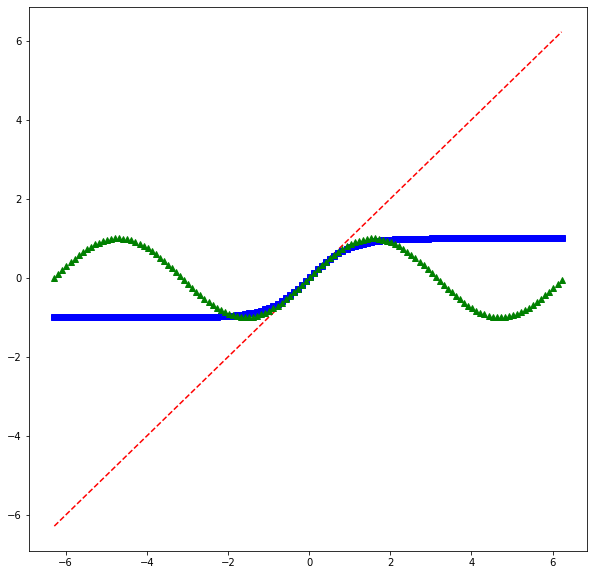
\includegraphics[width=\textwidth,height=0.6\textheight,keepaspectratio]{figures/Plot.png}\\
        \end{center}
        more at \href{https://matplotlib.org/stable/api/_as_gen/matplotlib.pyplot.plot.html}{matplotlib.pyplot.plot}
    \end{frame}
    \begin{frame}[fragile]{Matplotlib: Line Plot}
        \begin{itemize}
            \item Line plot is a basic plot type in \textbf{matplotlib}.
            \item It is used to visualize the relationship between two variables.
        \end{itemize}
    \end{frame}

    \begin{frame}[fragile]{Matplotlib: Scatter Plot}
        matplotlib.pyplot.\textbf{scatter}(x, y, s=None, c=None, marker=None, cmap=None, \dots, **kwargs)\\
        \begin{center}
            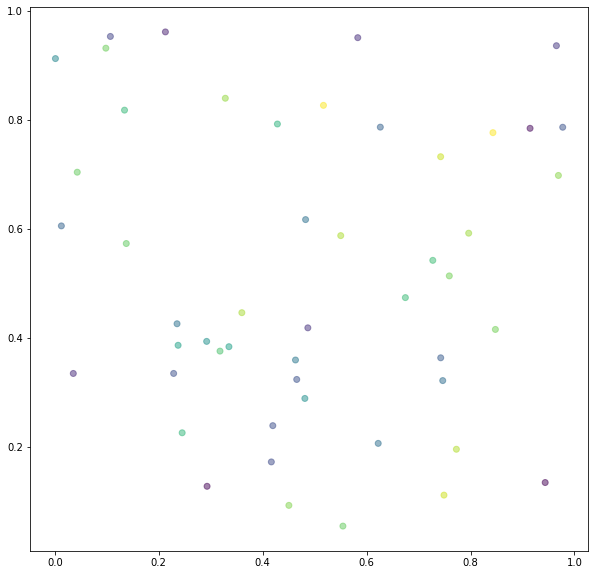
\includegraphics[width=\textwidth,height=0.6\textheight,keepaspectratio]{figures/Scatter.png}\\
        \end{center}
        more at \href{https://matplotlib.org/stable/api/_as_gen/matplotlib.pyplot.scatter.html}{matplotlib.pyplot.scatter}
    \end{frame}
    \begin{frame}[fragile]{Matplotlib: Scatter Plot}
        \begin{itemize}
            \item Scatter plot is used to visualize the spatial relationship between two variables.
            \item Each point in the scatter plot represents an observation in the dataset.
            \item Scatter plots are useful for identifying patterns, trends, and outliers in the data.
        \end{itemize}
    \end{frame}

    \begin{frame}[fragile]{Matplotlib: Box \& Whisker Plot}
        matplotlib.pyplot.\textbf{boxplot}x, vert=None, positions=None, widths=None, patch_artist=None, \dots, **kwargs)\\
        \begin{center}
            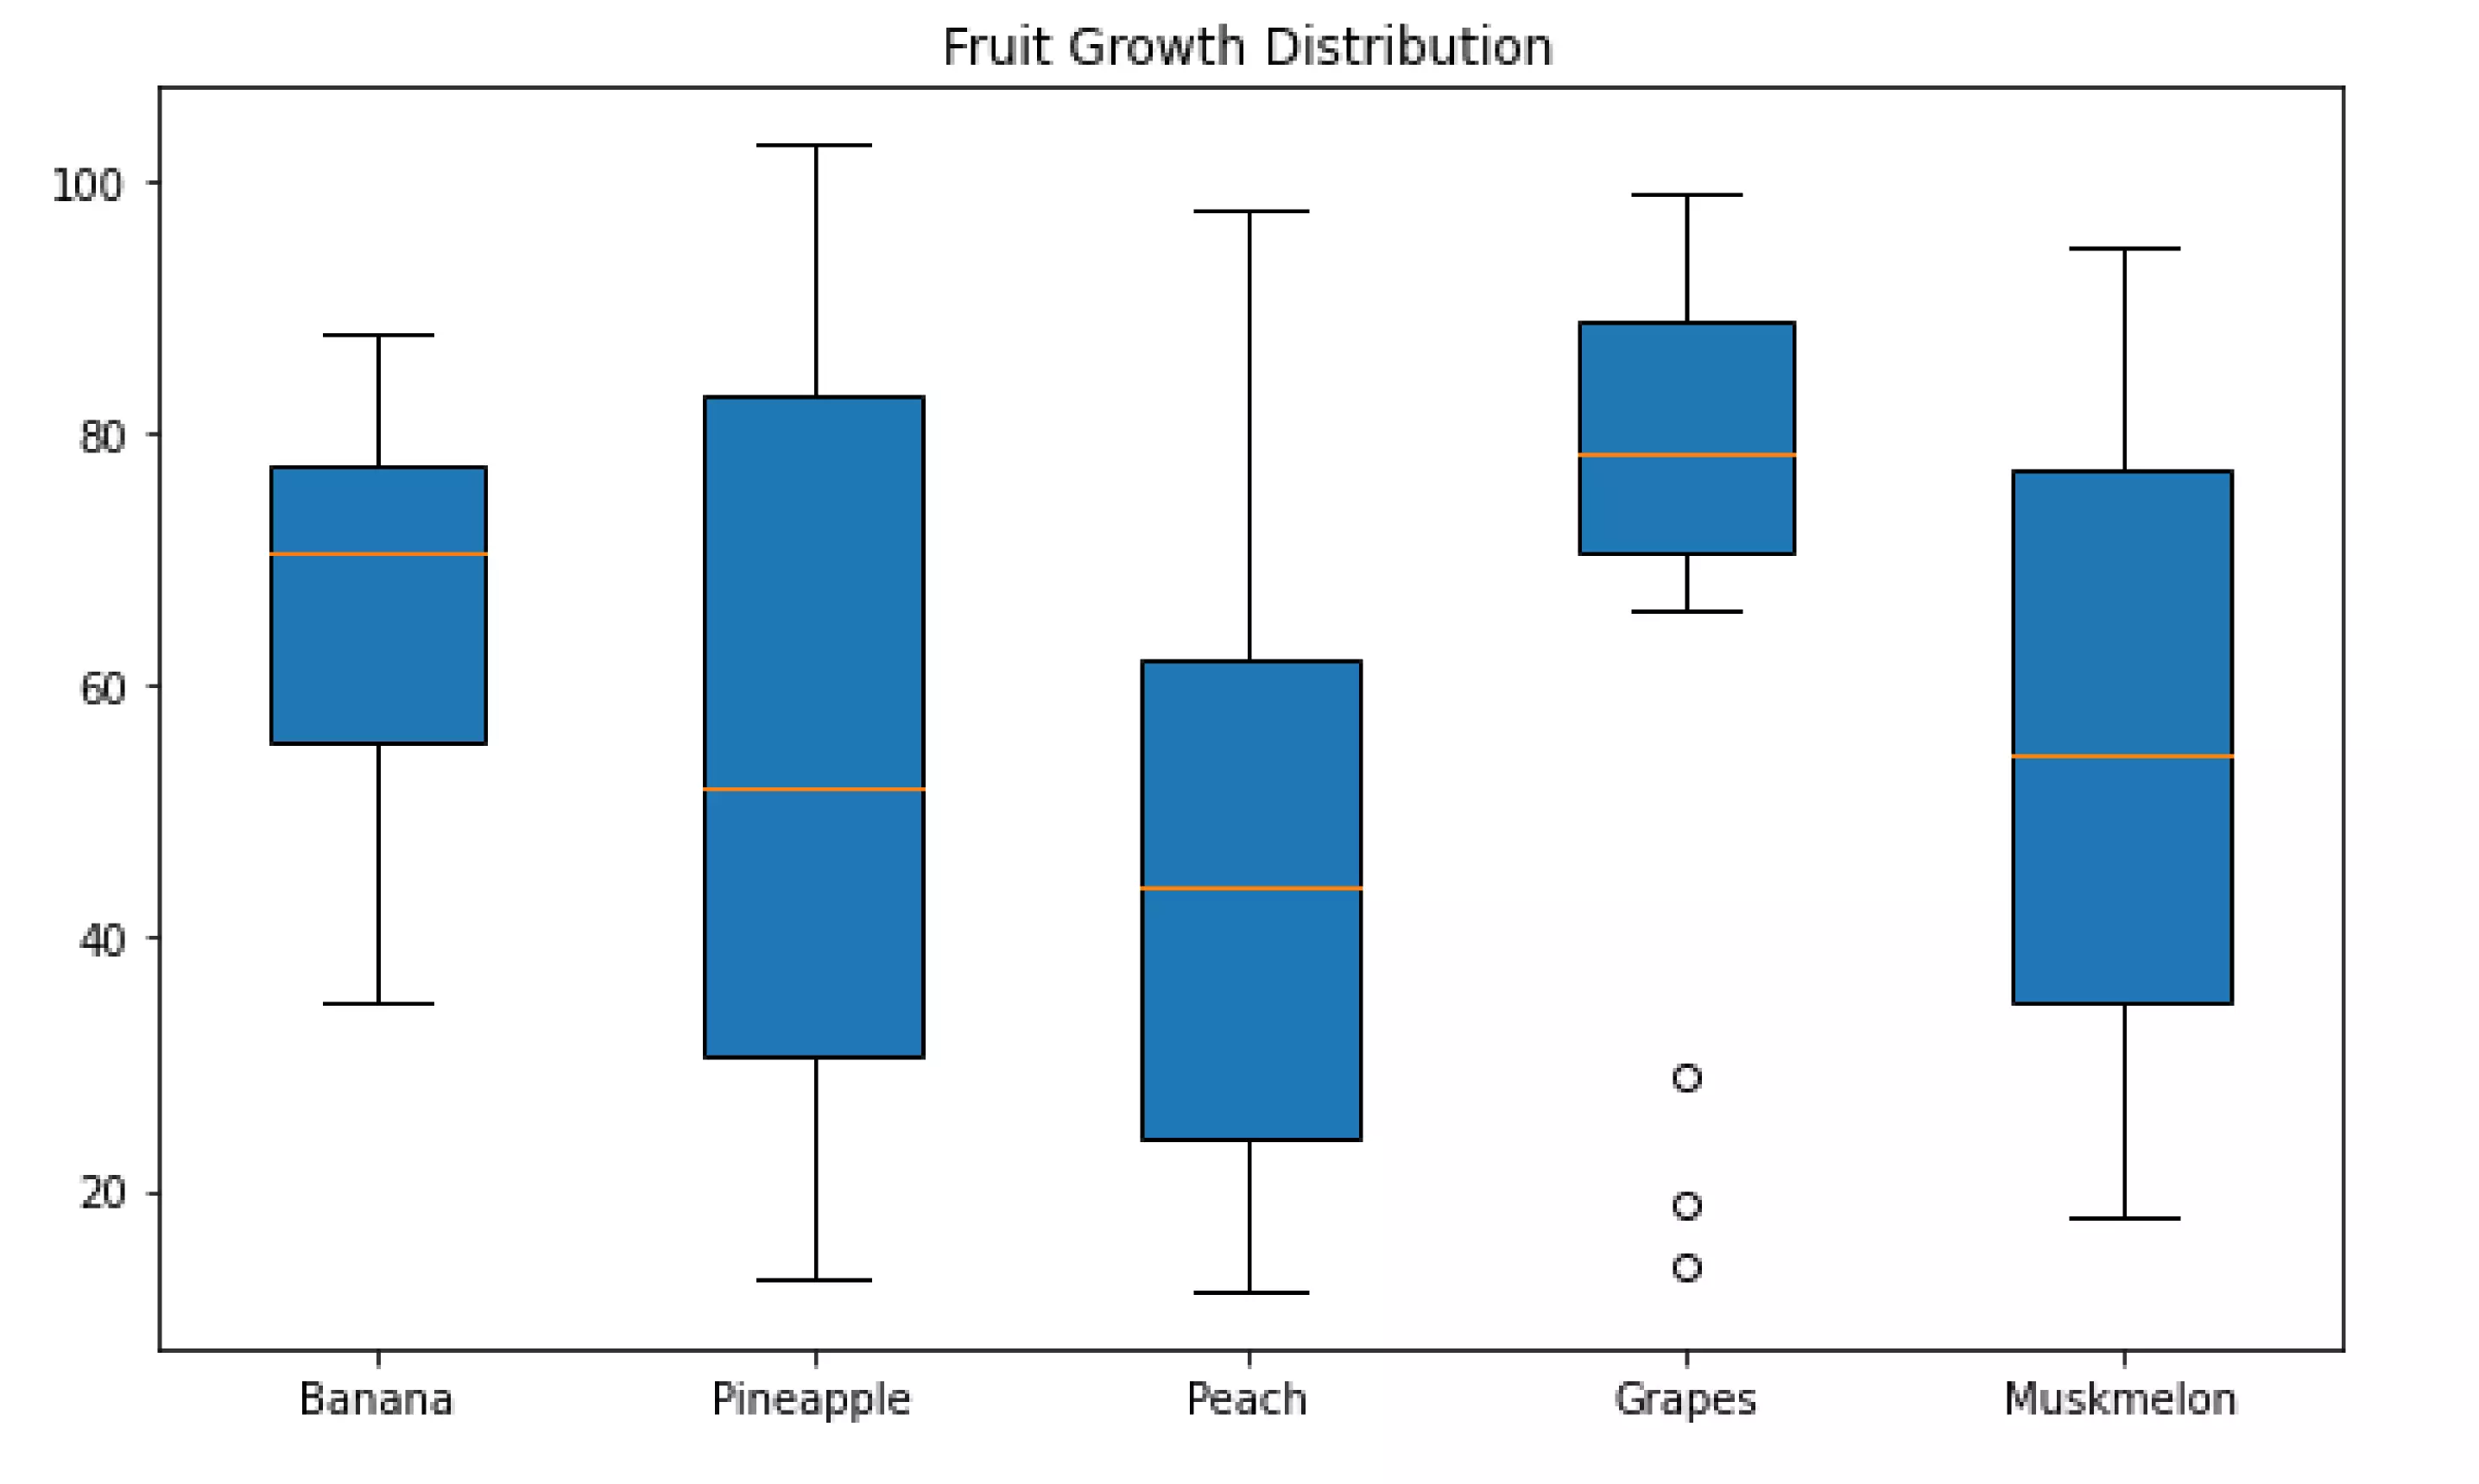
\includegraphics[width=\textwidth,height=0.6\textheight,keepaspectratio]{figures/boxplot.png}\\
        \end{center}
        more at \href{https://matplotlib.org/stable/api/_as_gen/matplotlib.pyplot.hist.html}{matplotlib.pyplot.hist}
    \end{frame}
    \begin{frame}
        \frametitle{Box \& Whisker Plot}
        \begin{itemize}
            \item Box and whisker plot is used to visualize the distribution of a dataset.
            \item It shows the median, quartiles, and outliers of the data.
            \item Box and whisker plots are useful for comparing distributions between different groups.
        \end{itemize}
    \end{frame}

    \begin{frame}[fragile]{Matplotlib: Violin Plot}
        matplotlib.pyplot.\textbf{violinplot}(dataset, positions=None, vert=True, widths=0.8, showmeans=False, \dots, **kwargs)\\
        \begin{center}
            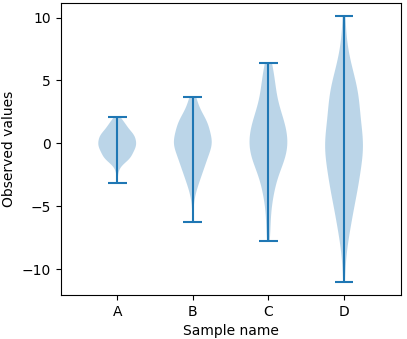
\includegraphics[width=\textwidth,height=0.6\textheight,keepaspectratio]{figures/violinplot.png}\\
        \end{center}
        more at \href{https://matplotlib.org/stable/api/_as_gen/matplotlib.pyplot.violinplot.html}{matplotlib.pyplot.violinplot}
    \end{frame}
    \begin{frame}
        \frametitle{Violin Plot}
        \begin{itemize}
            \item Violin plot is used to visualize the distribution of a dataset.
            \item It combines the features of a box plot and a density plot.
            \item Violin plots are useful for comparing distributions between different groups.
        \end{itemize}
    \end{frame}

    \begin{frame}[fragile]{Matplotlib: Bar Plot}
        matplotlib.pyplot.\textbf{bar}(x, height, width=0.8, bottom=None, align='center', \dots, **kwargs)\\
        \begin{center}
            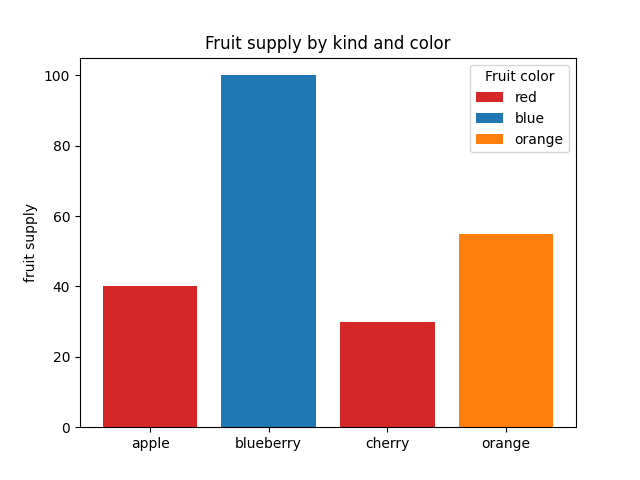
\includegraphics[width=\textwidth,height=0.6\textheight,keepaspectratio]{figures/bar.png}\\
        \end{center}
        more at \href{https://matplotlib.org/stable/api/_as_gen/matplotlib.pyplot.bar.html}{matplotlib.pyplot.bar}
    \end{frame}

    \begin{frame}[fragile]{Matplotlib: Histograms}
        matplotlib.pyplot.\textbf{hist}(x, bins=None, range=None, density=False, \dots, **kwargs)\\
        \begin{center}
            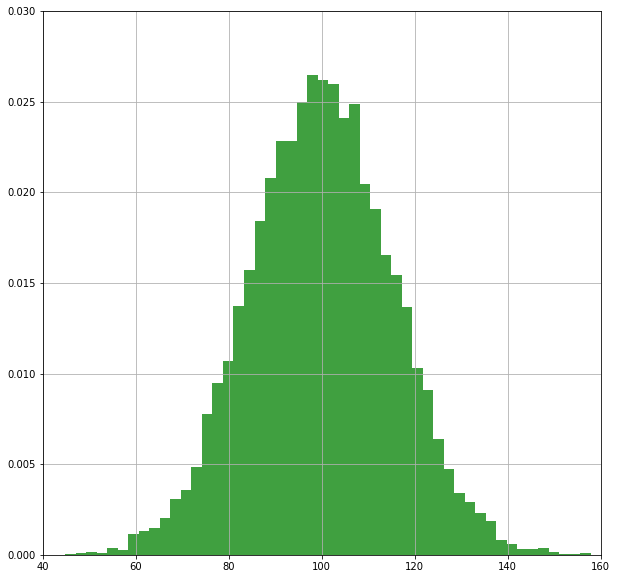
\includegraphics[width=\textwidth,height=0.6\textheight,keepaspectratio]{figures/Hist.png}\\
        \end{center}
        more at \href{https://matplotlib.org/stable/api/_as_gen/matplotlib.pyplot.hist.html}{matplotlib.pyplot.hist}
    \end{frame}
    \begin{frame}
        \frametitle{Histograms}
        \begin{itemize}
            \item Histograms are used to visualize the distribution of a dataset.
            \item They show the frequency of data points within specified ranges (bins).
            \item Histograms are useful for identifying the shape and spread of the data.
        \end{itemize}
    \end{frame}

    \begin{frame}[fragile]
        \frametitle{Histograms}
        \begin{lstlisting}[language=Python]
# Iterate over the ages and increment
# The corresponding bin count

for age in ages:
    if age < 30:
        bin_counts[0] += 1
    elif age < 40:
        bin_counts[1] += 1
    elif age < 50:
        bin_counts[2] += 1
    else:
        bin_counts[3] += 1

# Create a bar chart of the bin counts

plt.bar(bin_edges[:-1], bin_counts, width=10)
        \end{lstlisting}
    \end{frame}

    \begin{frame}[fragile]
        \frametitle{Histograms}
        \begin{lstlisting}[language=Python]
# Add labels and a title

plt.xlabel("Age")
plt.ylabel("Count")
plt.title("Age Distribution")

# Show the plot

plt.show()
        \end{lstlisting}
    \end{frame}

    \begin{frame}
        \frametitle{Histograms}
        \begin{center}
            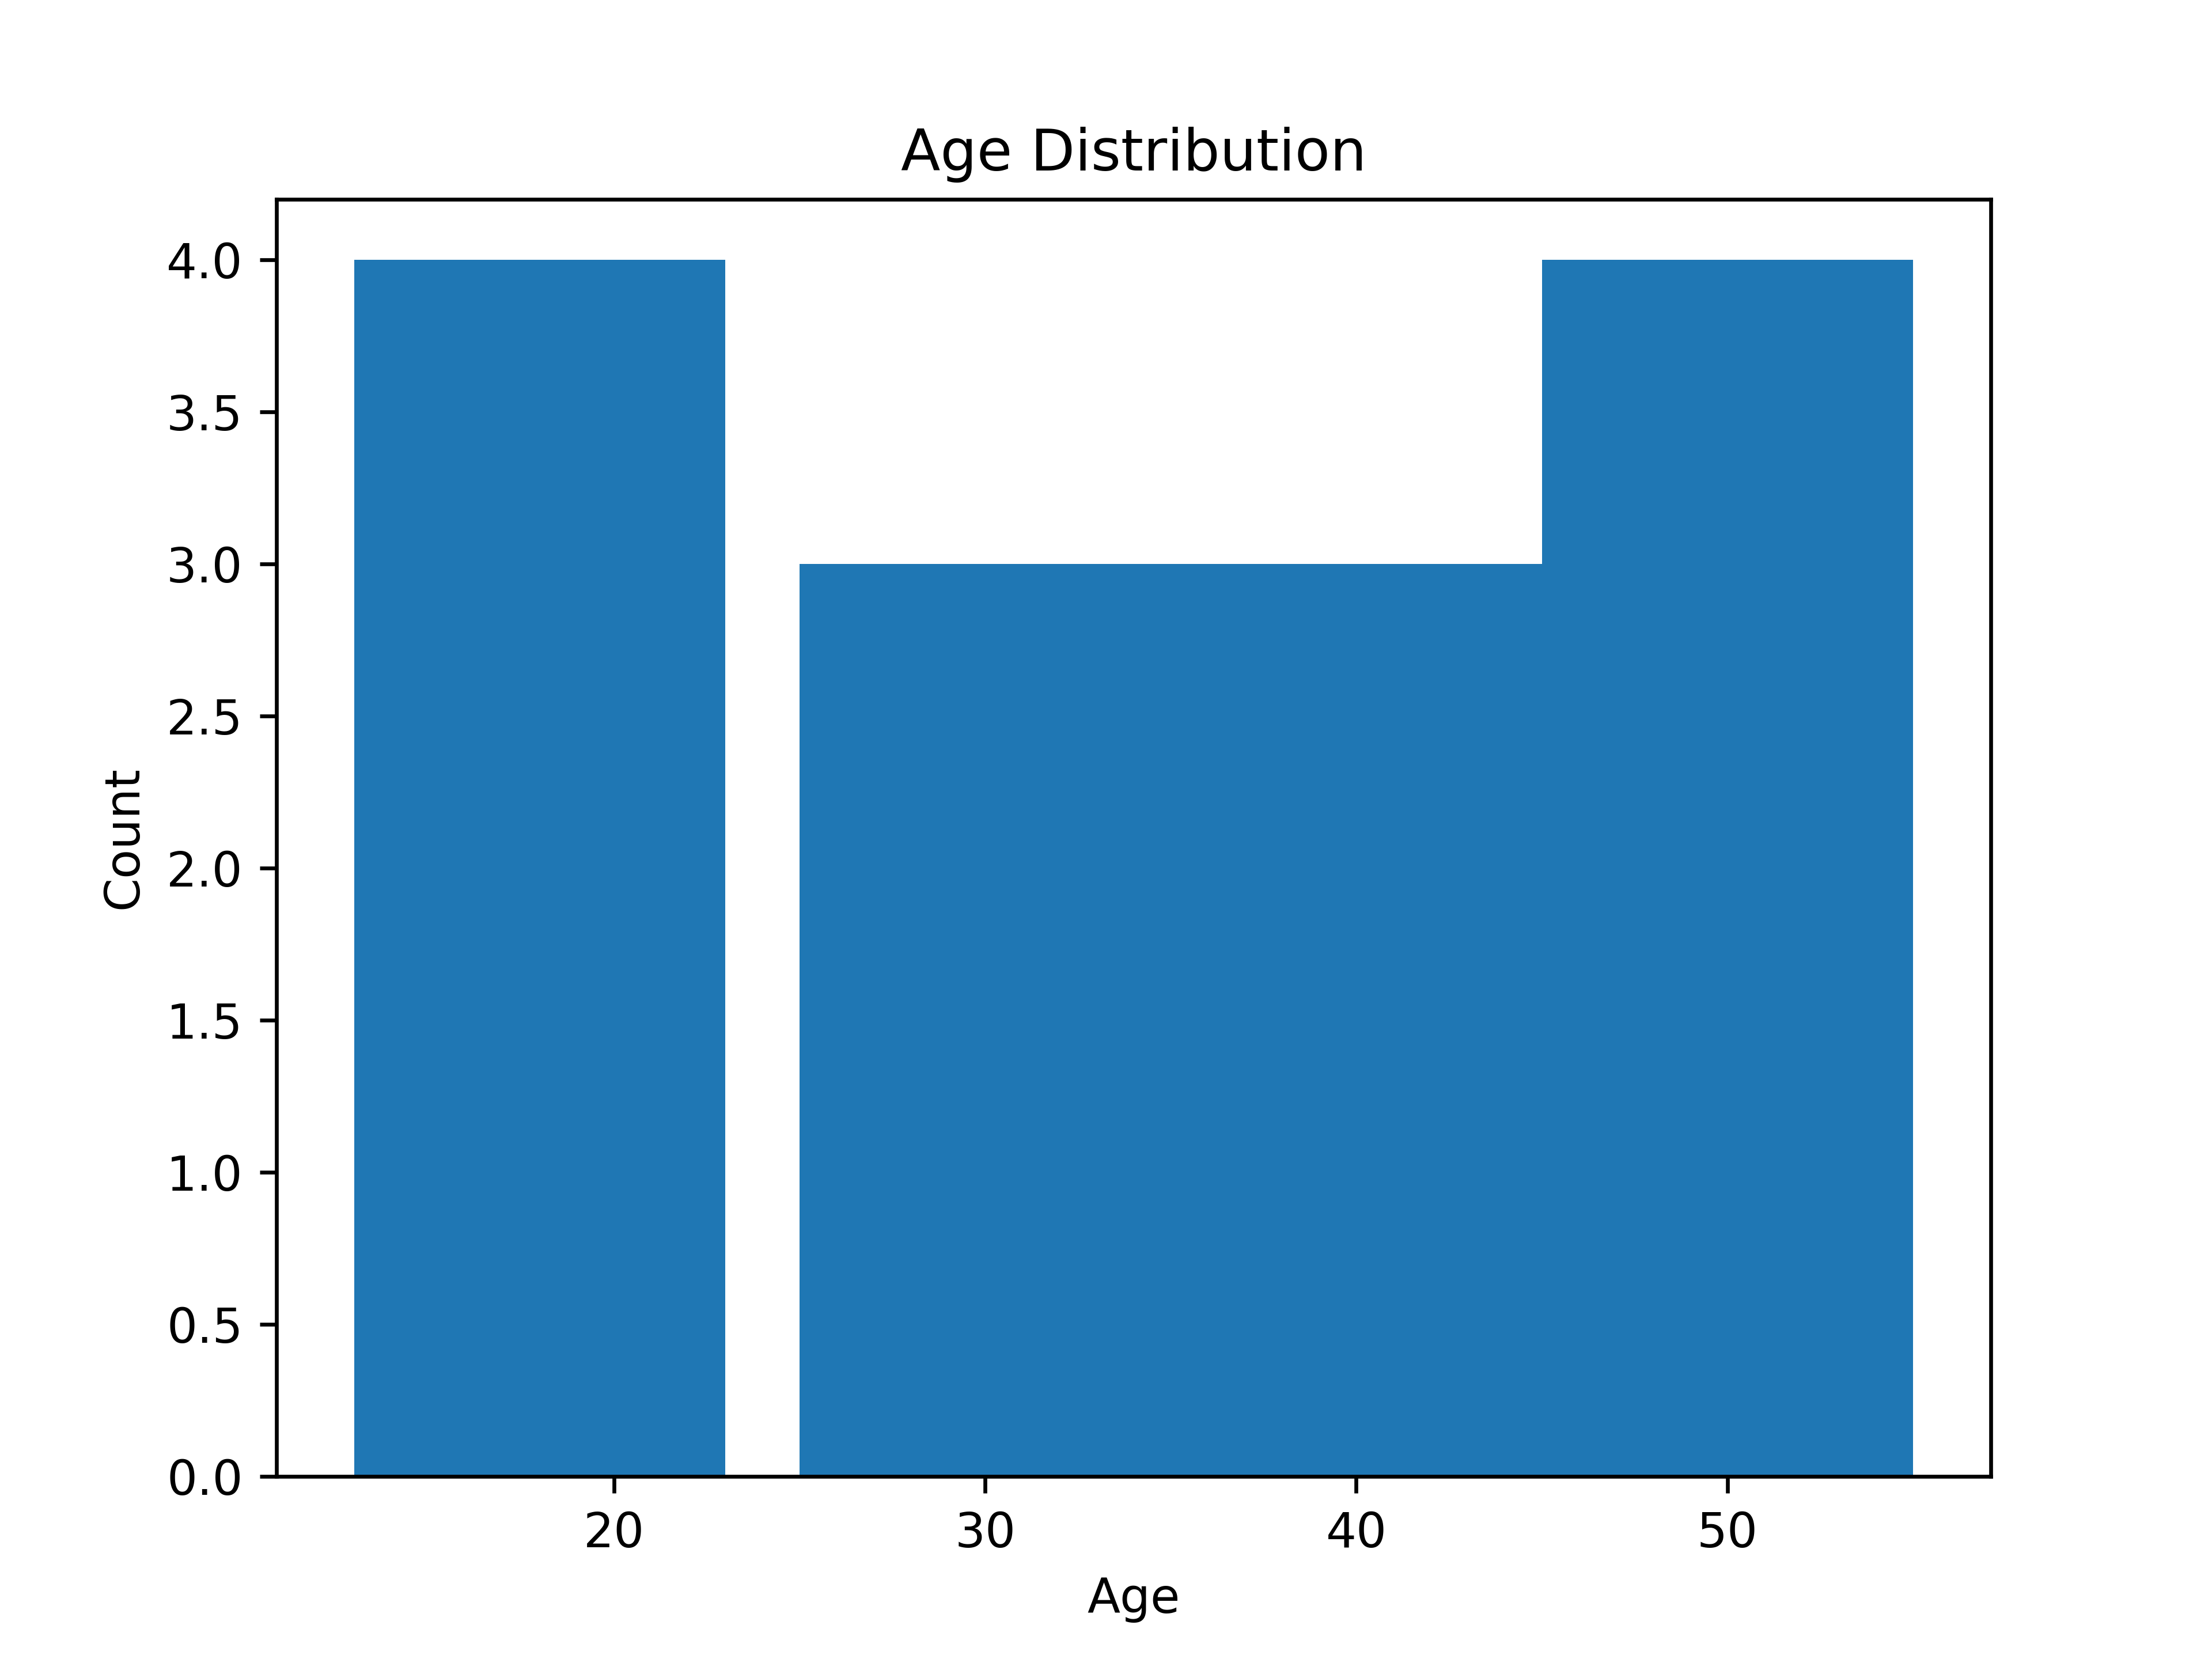
\includegraphics[width=0.7\linewidth]{figures/histogram_example_custom}
        \end{center}
    \end{frame}

    \begin{frame}[fragile]
        \frametitle{Box Plots}
        \begin{lstlisting}[language=Python]
import matplotlib.pyplot as plt

data.boxplot(column=['Column1', 'Column2', 'Column3'])
plt.ylabel('Value')
plt.title('Box Plots of Columns')
plt.show()
        \end{lstlisting}
    \end{frame}

    \begin{frame}[fragile]{Matplotlib: Plot styles}
        \begin{itemize}
            \item \textbf{Plot styles} consist of 3 elements in combinations: "[marker][line][color]" or [color][marker][line]
            \item For example:
            \begin{itemize}
                \item 'r--' means a red dashed line with no marker.
                \item 'bs' means blue square marker with no line.
                \item 'g\^' means green triangle marker with no line.
                \item 'k:' means a black dotted line with no marker.
                \item 'mX-' means magenta X-filled marker with a solid line.
            \end{itemize}
        \end{itemize}
    \end{frame}
\end{document}